
\documentclass[12pt]{article}
\usepackage[english]{babel}
\usepackage[utf8x]{inputenc}
\usepackage{amsmath}
\usepackage{graphicx}
\graphicspath{ {scrn/} }
\usepackage[colorinlistoftodos]{todonotes}

\begin{document}

\begin{titlepage}

\newcommand{\HRule}{\rule{\linewidth}{0.5mm}} % Defines a new command for the horizontal lines, change thickness here

\center % Center everything on the page
 
%----------------------------------------------------------------------------------------
%	HEADING SECTIONS
%----------------------------------------------------------------------------------------

\textsc{\Large UNIVERSITATEA TEHNICĂ A MOLDOVEI}\\[1cm] % Second title
\textsc{\Large Facultatea „Calculatoare, Informatică şi Microelectronică”}\\[0.5cm] % Third title
\textsc{\large Specialitatea : Tehnologii informationale}\\[0.5cm] % Minor heading 

\textsc{\large Disciplina : Medii interactive de dezvoltare a produselor soft}\\[1.5cm] % Minor heading 
\large Lucrarea de laborator nr.1\\[1cm]
%----------------------------------------------------------------------------------------
%	TITLE SECTION
%----------------------------------------------------------------------------------------

\HRule \\[0.4cm]
{ \huge \bfseries Version control systems}\\[0.2cm] % Title of the document
\HRule \\[3cm]
 
%----------------------------------------------------------------------------------------
%	AUTHOR SECTION
%----------------------------------------------------------------------------------------

\begin{minipage}{0.4\textwidth}
\begin{flushleft} \large
\emph{A efectuat:}\\
\emph{}\\
\emph{A verificat:}\\
\end{flushleft}
\end{minipage}
~
\begin{minipage}{0.4\textwidth}
\begin{flushright} \large
st. gr. TI-141 \\
\textsc{Levcenco Elena}\\ % Student's Name
\textsc{ Cojanu Irina} % Teacher's Name
\end{flushright}
\end{minipage}\\[3cm]

%----------------------------------------------------------------------------------------
%	DATE SECTION
%----------------------------------------------------------------------------------------

{\large \today}\\[2cm] % Date, change the \today to a set date if you want to be precise

%----------------------------------------------------------------------------------------

\vfill % Fill the rest of the page with whitespace

\end{titlepage}
\section{Scopul lucrarii:}
Studierea unui Version Control System și lucru cu versiunea CLI a acestuia.Examinarea intrucțiunilor de bază și lucru cu un repositoriu remote.
\section{Obiective:}
\begin{itemize}
\item Intelegerea si folosirea CLI (basic level)
\item Administrarea remote a masinilor linux machine folosind SSH (remote code editing)
\item Version Control Systems (git || bitbucket || mercurial || svn)
\end{itemize}
\section{Laboratory Requirements: folosind drept VSC github}
\label{sec:examples}

\subsection{Basic Level (nota 5 .. 6) :}
\begin{itemize}
\item initializeaza un nou repositoriu
\item configurarea VCS
\item crearea branch-urilor(cel putin 2 branches)
\item commit pe ambele branch-uri (cel putin 1 commit per branch)
\end{itemize}


\subsection{Normal Level (nota 7 .. 8):}
\begin{itemize}
\item setarea unui branch to track a remote origin pe care se face push (Github)
\item resetarea unui branch la commit-ul anterior
\item folosirea fisierului .gitignore
\end{itemize}
\subsection{Advanced Level (nota 9 .. 10):}
\begin{itemize}
\item merge 2 branches
\item rezolvarea conflictelor a 2 branches
\end{itemize}
\section{Concluzia:}
Primul pas este crearea unui repositoriu.Pentru aceasta dăm click pe + New Repository.
Următorul pas este alegerea unui nume pentru repository. Bifăm „Initialize this repository with a README”, alegem în partea de jos a paginii, adăugarea unui fișier .gitignore(Fisierele sau directoarele ce se doresc a fi ignorate de sistemul de versionare).
Pasul trei identificarea utilizatorului curent
Comenzi linie de comanda:\\
\begin{itemize}
\item git config user.name “Nume Utilizator”
\item git config user.email “email@gmail.com”
\end{itemize}
Sincronizarea cu repositoriul.Comenzi linie de comanda:
\begin{itemize}
\item git init (initializare workspace pentru GIT) 
\item git remote (asigura management-ul conexiunilor realizate cu repository-urile remote;
comenzi aditionale: add, -v [listare], rm, rename)
\item 
ssh-keygen -t rsa -b 4096 -C "email@gmail.com" \\
ssh-agent bash -c 'ssh-add /key; git clone git@github.com:ElenaLevcenco/MIDPS.git' (cloneaza un repositoriul)
\end{itemize}
Commit-erea
\begin{itemize}
\item git status (afiseaza o lista cu fisierele modificate fata de ultima versiune sincronizata)
\item git add text.txt undo.txt <...> (adaugarea de fisiere in cadrul versiunii ce se
intentioneaza a fi publicata)
\item git commit -m “primul commit” (demarcarea cu ajutorul unui mesaj a noi versiuni ce
urmeaza a fi publicata; commit-ul va avea atasat o versiune a reviziei [un hash], precum si
detaliile utilizatorului [identitatea lui])
\end{itemize}
Actualizarea versiunii curente a unui branch\\
Comenzi linie de comanda:
\begin{itemize}
\item git pull origin sensei
\end{itemize}
Migrarea intre branch-uri\\
\begin{itemize}
\item  git branch (va afisa branch-urile locale, precum si branch-ul curent pe care ne aflam)
\item git checkout guru (va schimba branch-ul curent in 'sensei',migrandu-se astfel pe un nou fir al versionarii)
\item  git checkout -b 'guru' sau git branch 'guru' (va crea un branch
nou pe baza celui curent)
\end{itemize}
Unirea a doua branch-uri\\Comenzi linie de comanda:
\begin{itemize}
\item git merge 'master' (va aplica modificarile din branch-ul specificat
branch-ului curent, daca acestea exista; branch-ul de unit poate fi atat local, cat si remote,
deci nesincronizat local)
\end{itemize}
Rezolvarea conflictelor:\\
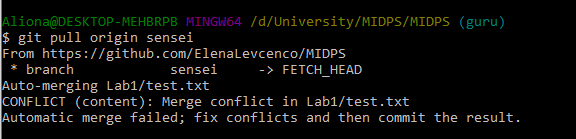
\includegraphics{conflict_detected.png}\\

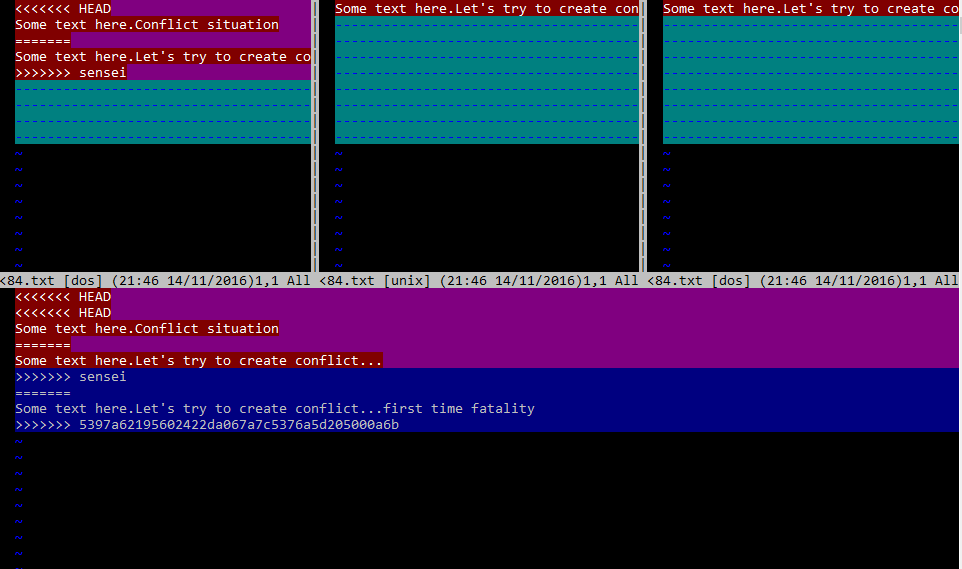
\includegraphics{conflict_text.png}\\

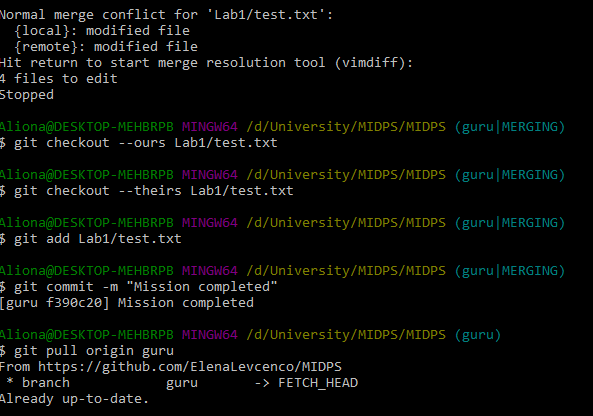
\includegraphics{resolve_conflict.png}\\

\section*{Concluzia}
Laboratorul dat isi propune insusirea comenzilor de baza a sistemului de versionare GIT de la linia de comanda.Sistemele de versionare permit gestionarea versiunilor multiple a unor fisiere, precum si asigurarea
lucrului colaborativ asupra acestor fisiere. Aceste sisteme au fost concepute pentru a permite membrilor mai multor echipe sa opereze
modificari pe acelasi proiect, aceste modificari urmand a fi reunite intr-o noua versiune a
proiectului.
\end{document}